\section{Experiments}

\noindent To explore the general effectiveness of our proposed soft-gating residual network for image generation tasks, we test on a variety of settings:

% \section{Experiments}
% We present the details of a set of experiments performed and the corresponding results of the experiments which show the efficacy of our Gated Residual Blocks albeit being simple to implement.

\begin{itemize}[noitemsep]
\item {1-D unconditional modeling}
% We show that individual blocks in a residual network self-organize into modes in a simple 1-D distribution.
\item {MNIST~\cite{XX} and FashionMNIST~\cite{XX} unconditional generation}
% We show that soft-gating can help improve generations in an InfoGAN setup.
\item {Outline$\rightarrow$Image class-conditional generation}
\item {Edges$\rightarrow$Handbags multimodal image generation}
\item {Disambiguating multiple disjoint tasks: Day$\rightarrow$Night and Cityscapes Label$\rightarrow$Image}
\end{itemize}

\subsection{Non Parametric Density Estimation:}

\paragraph{1D experiment}
We first evaluate the effect of a gating network in a simple scenario where the data distribution is a 1D mixture of Gaussians. 
We train \model{} in this simple setting, analyze the effect of removing different blocks via the gating network, in the vein of \cite{veit2016residual}.
We observe in Figure ~\ref{fig:onedexperiment}, when some residual blocks were disabled (and only the skip connection of that block was activated), it led to the disappearance of particular modes from the data distribution. 
Removal of groups of blocks led to the disappearance of clusters of modes from the generated distribution. 

In order to understand the behavior of the various residual blocks, we first perform a very simple synthetic experiment, much easier than generating high-dimensional complex images. We consider a distribution of 1D Gaussian Mixture \cite{bishop2007pattern} having five mixture components with modes at 10, 20, 60, 80 and 110, and standard deviations of 3, 3, 2, 2 and 1, respectively. While the first two modes overlap significantly, the fifth mode stands isolated as shown in \figref{fig:1d_ground}. We train our resnet block based GAN model using 1 million samples from this distribution and generate 1 million samples from the trained model. In order to compare the learned distribution with the ground truth distributions, we first estimate them using bins over the data points and create the histograms. These histograms are carefully created using different bin sizes and the best bin (found to be 0.1) is chosen. The generated distribution from the trained model corresponds very closely to the ground truth distribution \figref{fig:1d_gen}. The interesting aspect was that although the network was deeper (16 layers of residual blocks) than required for similar experiments in MAD-GAN \cite{ghosh2017multi}, Mode Regularized GAN \cite{che2016mode} and Unrolled GAN \cite{metz2017unrolledGAN}, there were only 4 neurons in each residual block with 16 layers of 4 neurons each in the generator and discriminator compared to fully connected versions in which there consisted of connections between 256 neurons in the preceding layer to 256 neurons in the current layer. Thus although the number of parameters were much less, the network learnt the distribution quite accurately.

The next set of experiments was the incision experiments similar to \cite{veit2016residual} on the generator after the network is trained. More specifically, if a layer (say $i^{th}$) had to be skipped, we disable the $f_i(x)$ of the ith residual block and now the output of the $i^{th}$ residual block is $x$ in place of the usual $x+f_i(x)$ encountered during training. Some interesting observations could be made, for example removing some blocks corresponded to the vanishing of certain modes from the generated distribution once the incision was performed on the generator network. Another surprising observation was that the same mode vanished on the incision of certain different residual blocks. This experiment validated the hypothesis of \cite{veit2016residual} that residual networks behave like an ensemble of several shallower networks and also pointed out that another network could predict based on the condition which blocks to use and to skip other non-necessary blocks in the network for that particular condition.


\subsection{InfoGAN based Model}
The intuitions gained from the experiments performed for the non-parametric density estimation led to the Gated Residual Block on the Generator of a GAN. InfoGAN \cite{chen2016infogan} presented a perfect setting to apply the Gated Residual Block in the case of the generator. The first set of experiments were on MNIST and Fashion-MNIST with sets of 10 discrete variables (since there were 10 classes in both of the datasets) and 2 continuous variables whose information was tried to be maximized using the Q network. As can be seen in \figref{fig:infogan_unconditional} the network was able to generate realistic images from the different classes and produce meaningful interpolations by varying the continuous variables as shown in the figure. The exact experimental setting was that the hypernetwork responsible for the predictions of the $alpha^i$s which we term as the gate selection network gets the salient variables and has no information about the random noise sampled for the main network(consisting of gated residual blocks), based on the salient variables received the gate selection network predicts the  $alpha^i$s for all the blocks of the network. The main network is oblivious of the conditioning received in the salient variables and has to generate images coherent with the conditioning since the Q-Network tries to reconstruct back the conditioning received in the form of salient variables. 

\begin{figure}[t]%[ht!]
    \centering
    \addSubFigHalf{Picture35}{MNIST}{fig:infogan_mnist} 
    \addSubFigHalf{Picture34}{Fashion-MNIST}{fig:infogan_fashion_mnist} 
    \caption{Gated Residual Block-InfoGAN on MNIST and Fashion MNIST \ow{do we have the standard infogan comparison here?}}
    \label{fig:infogan_unconditional}
    \vspace{-3mm}
\end{figure}

\subsection{Unconditional Generations}
\begin{figure}[t]
    \centering
    \includegraphics[width=0.5\linewidth]{Picture5}
    \caption{Results on the Gated Residual Block on MNIST dataset}\label{fig:grb_mnist}
    \vspace{-4mm}
\end{figure}

A well known problem in image conditional GAN settings is the tendency to produce realistic outputs but not being able to produce meaningful variations in the generated output. It was especially prevalent in the original pix2pix setting \cite{isola2016image2image} and further research enabled variations such as \cite{ghosh2017multi} and \cite{zhu2017toward}. Although as shown in \cite{ghosh2017multi} the naive infoGAN setting couldn't produce meaningful variations in the pix2pix setting, settling rather for very minute variations. Our Gated Residual Blocks could mitigate some of the problems and did produce variations in the challenging task of edges-to-bag generation as has been demonstrated in \figref{fig:infogan_bags}. By varying the continuous variable smooth interpolations could be obtained between colors and textures which was earlier not possible with the infogan based pix2pix setting. Although the variations along the discrete axis was quite minimal and we are still investigating the cause for the same. The experimental setting in this scenario was that the salient variables were only given to the gate selection network and had to predict the $alpha^i$s for the main network which consisted of gated residual blocks and was oblivious of the conditioning provided in the form of salient variables. The Discriminator network was the standard image conditional discriminator network while the Q network in this scenario was modified to take the generated image as well as the edge map to behave as a image conditional Q Network which tries to reconstruct back the salient variables given to the gate selection network. 

\newcommand{\addSubFigEighth}[3]{\begin{subfigure}[t]{.18\linewidth}
   \includegraphics[width=\linewidth]{#1}
   \caption{#2}\label{#3}\end{subfigure}
}
\newcommand{\addSubFigEighthCaptionless}[3]{\begin{subfigure}[t]{.18\linewidth}
   \includegraphics[width=\linewidth]{#1}
   \label{#2}\end{subfigure}
}
\begin{figure*}[t]%[ht!]
    \centering
    \addSubFigEighthCaptionless{Picture8}{Sketch}{fig:bag_sketch} 
    \addSubFigEighthCaptionless{Picture9}{Varition 1}{fig:bag_1} 
    \addSubFigEighthCaptionless{Picture10}{Varition 2}{fig:bag_2}
    \addSubFigEighthCaptionless{Picture11}{Varition 3}{fig:bag_3}
    \addSubFigEighthCaptionless{Picture12}{Varition 4}{fig:bag_4}
    \caption{The variations produced in the sketch to realistic bag task in the infogan with Gated Residual Block setting for the generator }
    \label{fig:infogan_bags}
    \vspace{-3mm}
\end{figure*}

The next set of experiments were performed to judge the robustness of the Gate Selection Blocks and the Gated Residual Blocks in the case the labels were available. That meant using the gate selection network and the gated residual blocks on the discriminator. The implications were even more interesting, the gate selection network would have to distribute the blocks between the classes to get the class specific gradients back for training the class conditioned generator. In the unconditional setting for the generator, the main block only receives random noise and the gate selection block receives the class condition and predicts the $aplha^i$s for the gated residual blocks. The discriminator on the other hand is composed of a main network consisting of gated residual blocks which is oblivious to the class conditioning and a gate selection network which predicts the $aplha^i$s for the main network of the discriminator. The main network predicts how real/fake an image is based on the alpha weightings of its gated residual blocks. The network is able to disentangle the class conditioning although none of the main networks of the generator/ discriminator are aware of the class conditioning, the class information only being input to the gate selection network which has to modulate the weights of the respective networks' gated residual blocks. The generated samples on the MNIST dataset are shown in \figref{fig:grb_mnist} and the alpha gatings for the different classes and the different blocks in \figref{fig:mnist_act}. The values for the gates clearly show switching off of certain blocks in the case it is not needed for a particular class even though a sparsity constraint was not applied in the training objective.


\begin{figure}%[ht!]
    \centering
    \addSubFigHalf{Picture6}{Activations of the gated residual blocks in the generator}{fig:gen_act} 
    \addSubFigHalf{Picture7}{Activations of the gated residual blocks in the discriminator}{fig:dis_act} 
    \caption{Activation of the various blocks in the Generator and Discriminator}
    \label{fig:mnist_act}
    \vspace{-3mm}
\end{figure}


\subsection{Image Conditional Generations}

\paragraph{Scribble Dataset:}
To test the capability of our techniques on the varied kinds of generation tasks, we collected a dataset of 10 classes with 150 images each from each class. We obtained the scribbles using Adobe Photoshop's tool for outlining objects. We further had a test set consisting of 50 images for each class. The classes collected were basketball,chicken,cookie,cupcake,moon,orange,soccer,strawberry, watermelon, pineapple. 

\paragraph{Network Architecture}
\rz{shorten this into a few sentences for each net, so reader knows what we tested later, and point to suppmat where the tables can go}

\paragraph{Skinny ResNet}

The incision experiments as performed by \cite{veit2016residual} showed that deeper networks have more  valid paths of computation. Our incision experiments on the 1D Mixture of Gaussians setting also demonstrated the effectiveness of having deeper residual networks with lesser number of neurons in each block. We therefore design a network architecture which doesn't change the number of channels even in the case where the spatial resolution changes since the gating is applied to all the blocks including the downsampling and upsampling residual blocks and the hypothesis is that the gating mechanism would work best if all the blocks had similar number of modulations per block.

\paragraph{Encoder-Decoder} As a baseline, we test the encoder-decoder architecture from MUNIT~\cite{huang2018multimodal} which consists of an encoder followed by a set of residual blocks with a decoder at the end. 


\begin{figure*}[h]
    \centering
    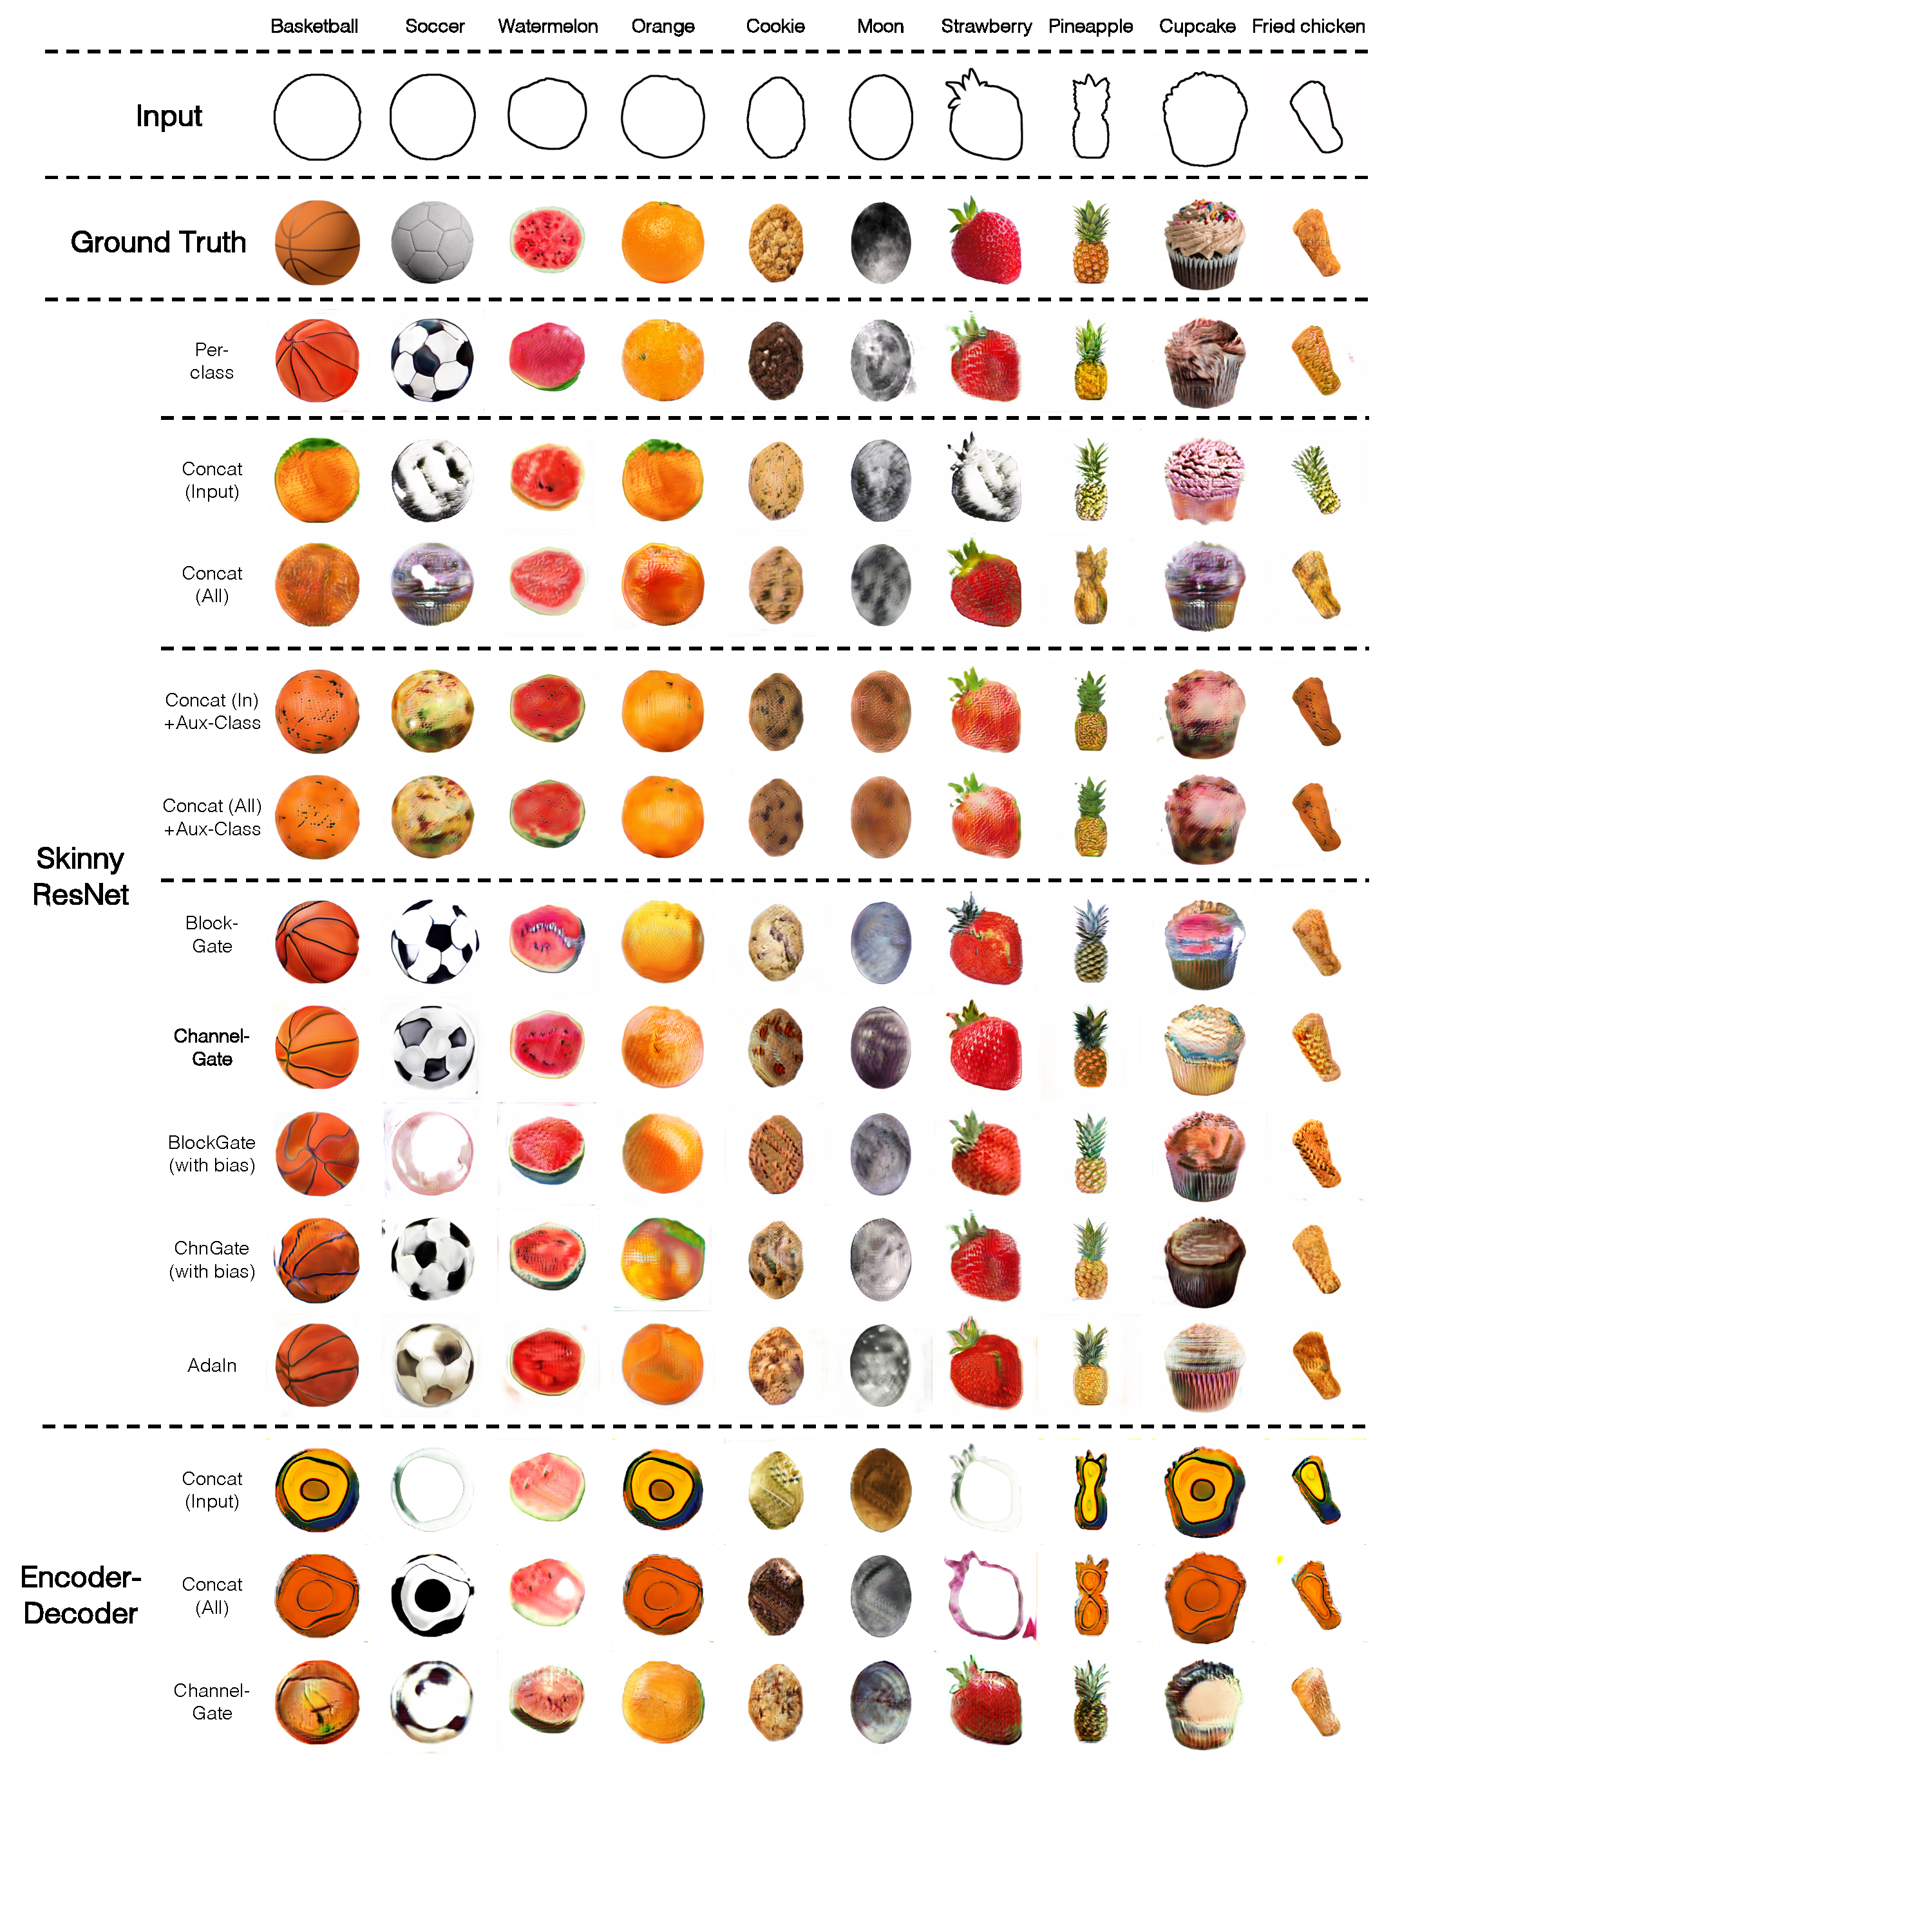
\includegraphics[width=.9\linewidth]{paper_images/cond_comp2.pdf}
    \caption{{\bf Algorithm Comparison} \label{fig:alg_comp} }
    \vspace{-4mm}
\end{figure*}

The task involves multiple different objects of high realism when the input is very similar for the various classes several of them being exactly same(in the case of circular objects where the input scribble is an identical scribble for all circular classes). As we can see from the generations \figref{fig:alg_comp} all of the various gating mechanisms and the baselines are able to generate images of high quality and realism from some classes but most of the baselines fail in some class and confuses with some other class. The gating mechanism on the other hand succeeds in separating out the various classes and doesn't confuse the class specific generations. Among the gating mechanisms channel wise gating has the best realism which is also corroborated by the Amazon Mechanical Turk Experiments and the classification accuracy of an Inception network finetuned on our dataset demonstrates the purity of the generations corresponding to the correct class using the gating mechanism.  

% \begin{figure}
%     \centering
%     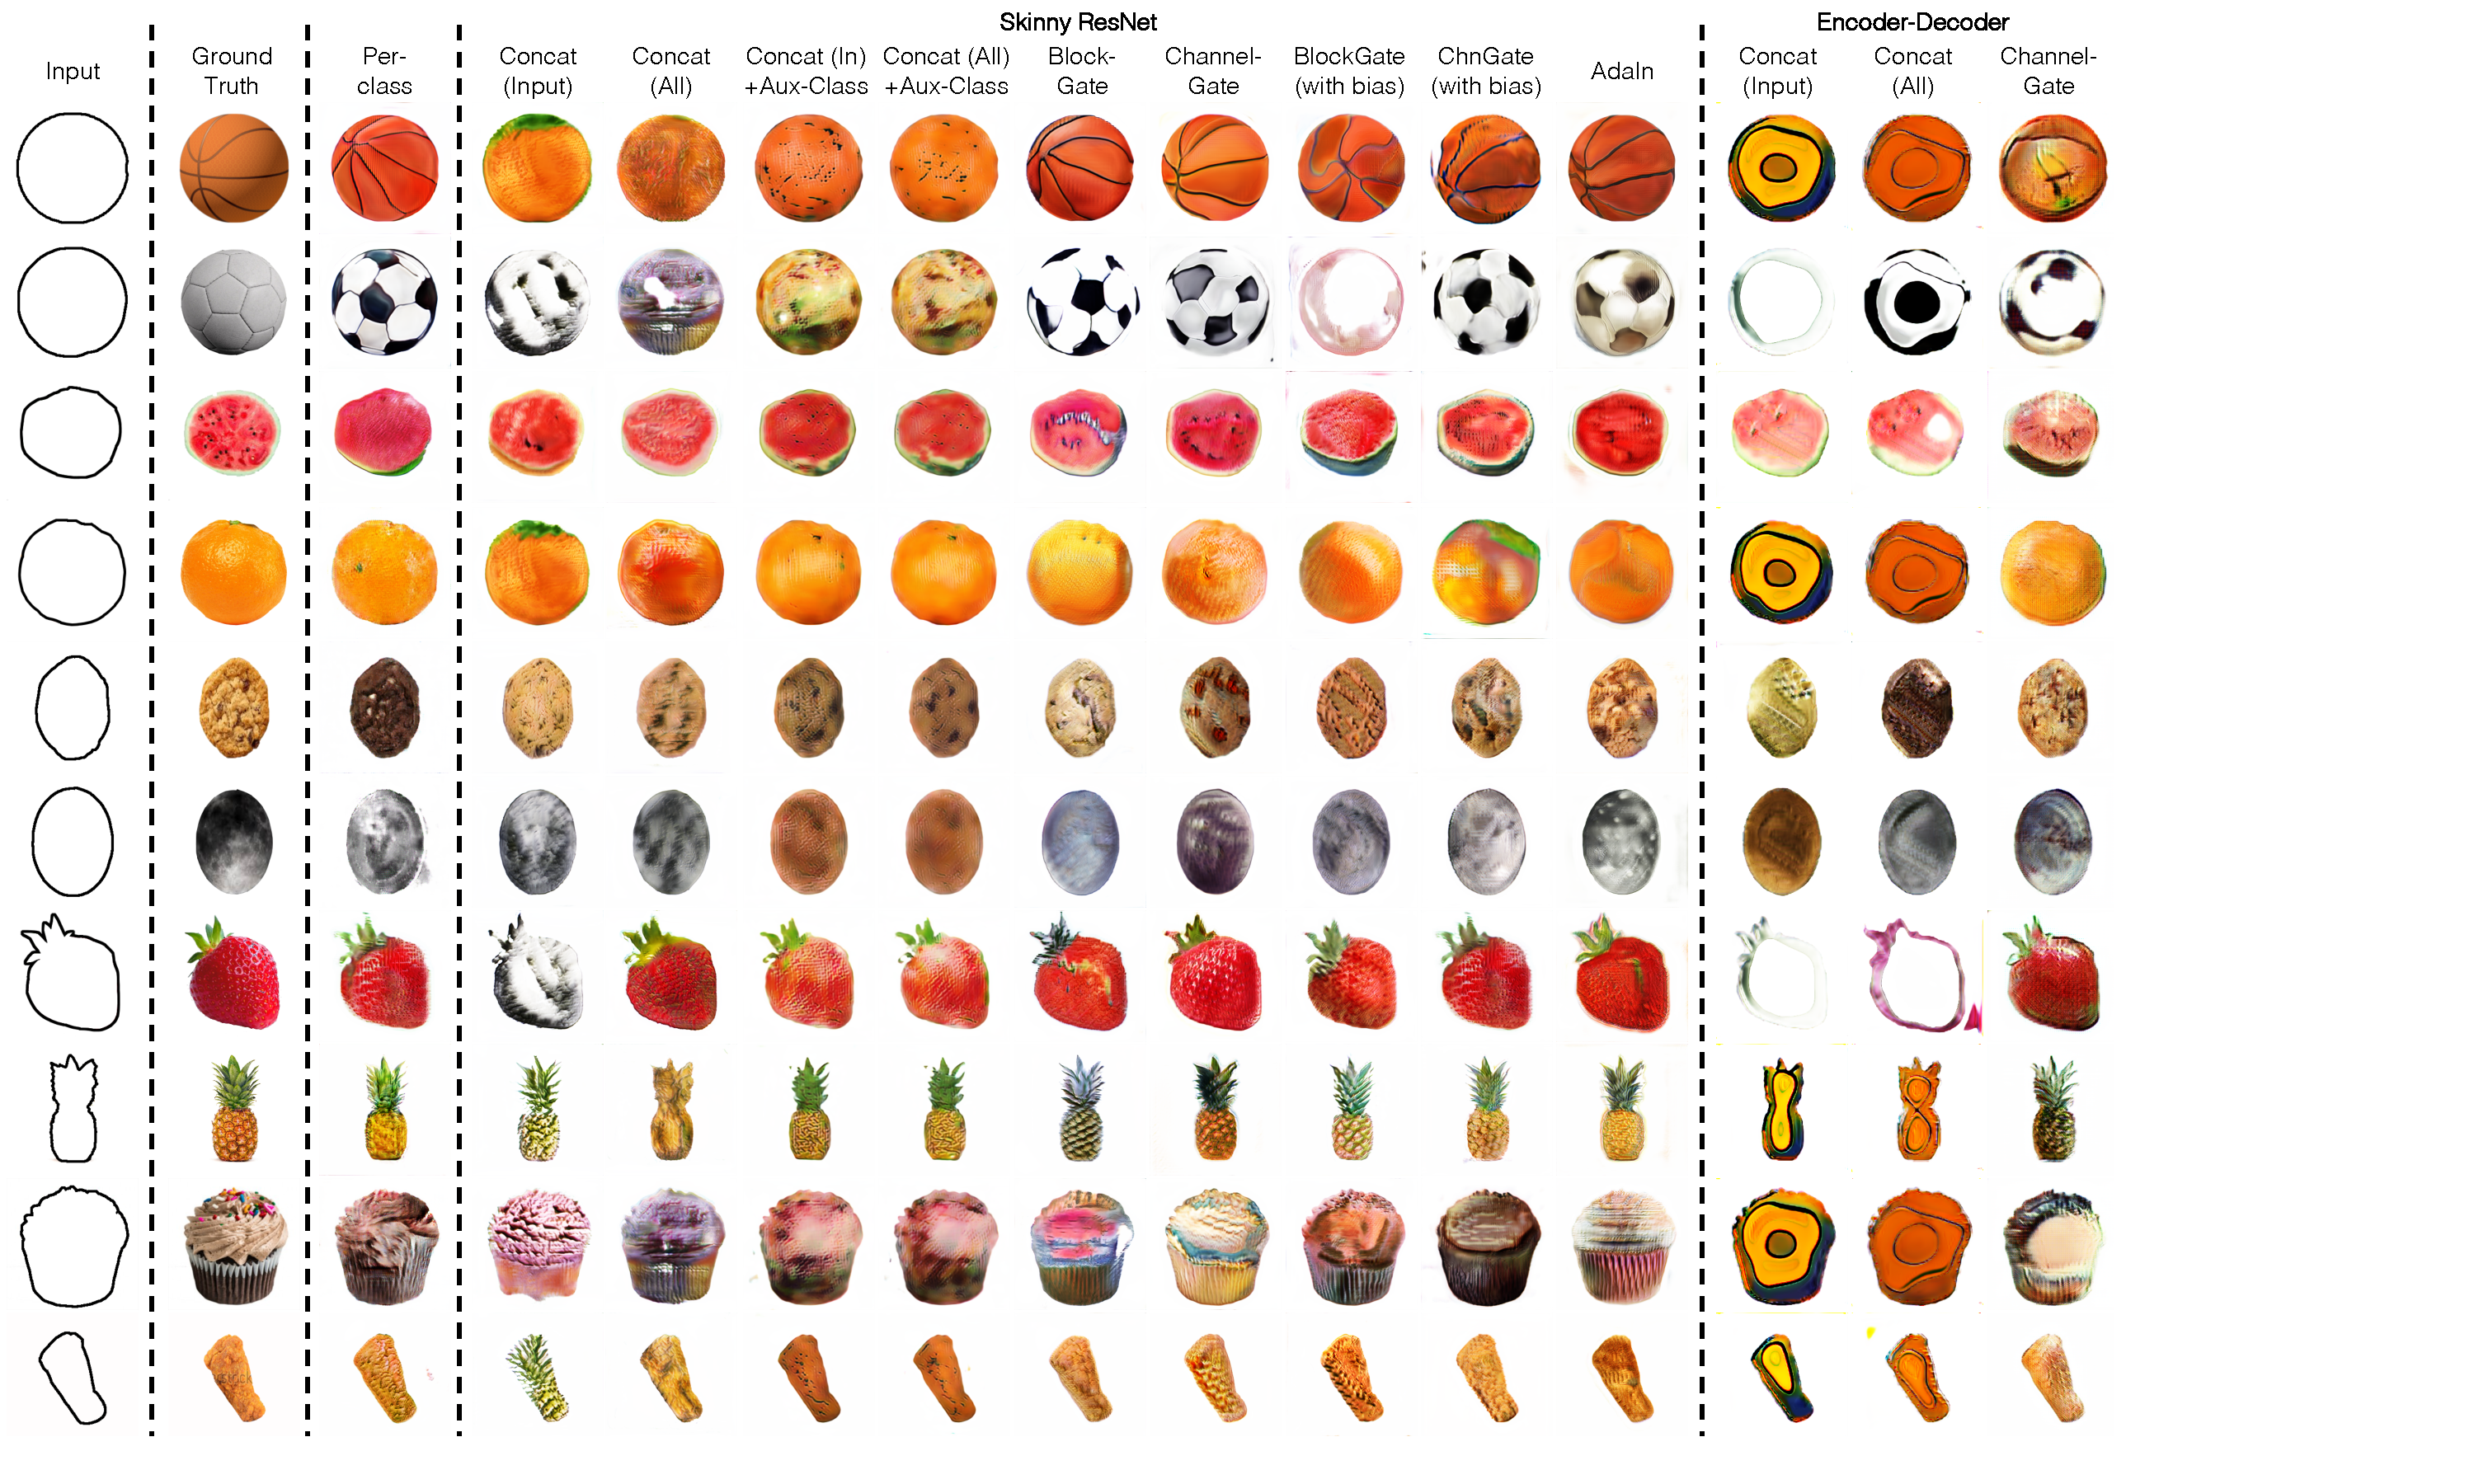
\includegraphics[width=\linewidth]{paper_images/cond_comp.pdf}
%     \caption{Algorithm Comparison}\label{fig:conditioning_amt}
% \end{figure}

% In the widely popular image conditioned generative models introduced in Pix2pix by \cite{isola2016image2image} although the results are brilliant, it had the inherent problem of only being applicable to a particular task such as different networks had to be trained for edges to shoes and edges to handbags, although StarGAN \cite{choi2017stargan} mitigated some of the problems but it was only applicable for relatively minute transformations such as changing the characteristics of the face.

% To analyze properly the task of multi-class generations in the image conditioned setting we introduce a new task of generating class conditioned realistic images from very rough scribbles. We start off with 3 classes, namely: pizza, strawberry and oranges. A simple pix2pix network fails to identify the different classes and starts injecting weird textures such as pizza on orange or strawberry on pizza as depicted in the results from pix2pix on this task in \figref{fig:scribble_pix2pix}. 

% In the conditional setting for the generator, the main block only receives the input scribble and the gate selection block receives the class condition and predicts the $aplha^i$s for the gated residual blocks. The discriminator on the other hand is composed of a main network consisting of gated residual blocks which is oblivious to the class conditioning and a gate selection network which predicts the $aplha^i$s for the main network of the discriminator. The main network also receives the input scribble alongside the generated/real image to predict how real/fake an image is based on the alpha weightings of its gated residual blocks. The network is able to disentangle the class conditioning although none of the main networks of the generator/ discriminator are aware of the class conditioning, the class information only being input to the gate selection network which has to modulate the weights of the respective networks' gated residual blocks. The results of the model are depicted in \figref{fig:scribble_grb} whereby we can clearly see that the network has been able to disentangle the class conditioning and generate textures appropriate for the right class.


% \subsection{Comparison to other forms of conditioning in Resblock :}
% Conditional Batch Normalization, FiLM and Adaptive Instance Normalization are the techniques which are the most closely related to our methodology. All of these have the benefit of being applicable even without the presence of residual blocks in the architecture. So an exhaustive comparison with all of these methods along with our form of conditioning on the residual blocks is a valid set of experimentation and has to be done to make the paper complete.

% \begin{figure}
%     \centering
%     \includegraphics[width=\linewidth]{conditioning_amt.png}
%     \caption{AMT studies of the various gating techniques on the scribble dataset}\label{fig:conditioning_amt}
%     \vspace{-4mm}
% \end{figure}
\begin{figure}
    \centering
    \includegraphics[width=\linewidth]{paper_images/gen_real_vs_acc.pdf}
    \caption{Generation realism vs accuracy}\label{fig:conditioning_amt}
    % \vspace{-4mm}
\end{figure}



\subsection{Infogan Variations(pix2pix):}
In the pix2pix setting as shown by previous works \cite{ghosh2017multi} and \cite{zhu2017toward} even the InfoGAN setup wasn't able to produce meaningful variations in the generations and needed different generators or 2 cycles respectively to produce meaningful variations in the generated images. With our best gating mechanism (Channel wise multiplication), it leads to meaningful variations albeit might be lesser than the other 2 methods \cite{ghosh2017multi} ,\cite{zhu2017toward}.

\begin{table}[ht]
\caption{Evaluation on Edges to Handbags diverse generations. Diversity using LPIPS metric \cite{zhang2018unreasonable}} % title of Table
\small
\centering % used for centering table
% \begin{tabular}{|c|c|c|c|} % centered columns (4 columns)
\begin{tabular}{p{3cm}p{3cm}} % centered columns (4 columns)
% \hline
\toprule
\textbf{Model} & \textbf{LPIPS Distance} \\%heading
\midrule
BicycleGAN \cite{zhu2017toward} & $0.1374 \pm 0.0005$  \\ % inserting body of the table
\midrule
Ours(Gated) & $0.0964 \pm 0.0003$  \\
\midrule
Concat(Input) &  $0.0432 \pm 0.0002$ \\
\midrule
Concat(All Layers) & $0.0159 \pm 0.0004$ \\
\midrule
Random Real Images & $0.3665 \pm 0.0053$ \\
\bottomrule %inserts single line
\end{tabular}
\label{table:infogan_lpips} % is used to refer this table in the text
\end{table}


\begin{figure}
    \centering
    \includegraphics[width=\linewidth]{infogan.jpg}
    \caption{Naive Conditioning of infogan fails while gating succeeds}\label{fig:infogan_gate}
    \vspace{-4mm}
\end{figure}

\subsection{Multi-Task Generations: }
Since our network is robust enough to be able to generate images conditioned on class and modulation of which blocks to use, it can further be used to generate images which are different in tasks such as the same network could do both day2night and instance maps to realistic generations of street scenes. As we can see in \figref{fig:multi-task_cityscapes} our model (Gated,Channel) is able to perform both tasks while the other techniques focus on only 1 of them more. In case of MUNIT like architecture conditioned on all layers the discriminator became too powerful after a while and the training progressed with only the L1 loss which caused the blurry generations in the case of segmentation maps to real image synthesis as evident from the figure.


\begin{figure*}%[ht!]
\centering
\begin{tabular}{*{5}{c@{\hspace{3px}}}}
    \includegraphics[width=.18\linewidth]{channel_gated/cityscapes_95_real_A} &
    \includegraphics[width=.18\linewidth]{channel_gated/cityscapes_95_fake_B} &
    \includegraphics[width=.18\linewidth]{munit_baseline_all/cityscapes_95_fake_B} &
    \includegraphics[width=.18\linewidth]{our_baseline_all/cityscapes_95_fake_B} & 
    \includegraphics[width=.18\linewidth]{acgan_baseline_all/cityscapes_95_fake_B} \\
    
    \includegraphics[width=.18\linewidth]{channel_gated/night2day_58_5018_to_5000_real_A} &
    \includegraphics[width=.18\linewidth]{channel_gated/night2day_58_5018_to_5000_fake_B} &
    \includegraphics[width=.18\linewidth]{munit_baseline_all/night2day_58_5018_to_5000_fake_B} &
    \includegraphics[width=.18\linewidth]{our_baseline_all/night2day_58_5018_to_5000_fake_B} &
    \includegraphics[width=.18\linewidth]{acgan_baseline_all/night2day_58_5018_to_5000_fake_B} \\
    \small
    \begin{subfigure}[t]{.18\linewidth}\caption{Input}\label{fig:daynightinput}\end{subfigure} &
    \begin{subfigure}[t]{.18\linewidth}\caption{Ours}\label{fig:daynightinput}\end{subfigure} &
    \begin{subfigure}[t]{.18\linewidth}\caption{MUNIT Conditioning All Layers}\label{fig:daynightinput}\end{subfigure} &
    \begin{subfigure}[t]{.18\linewidth}\caption{Our Conditioning All Layers}\label{fig:daynightinput}\end{subfigure} &
    \begin{subfigure}[t]{.18\linewidth}\caption{ACAN (our Architecture Conditioning all layers)}\label{fig:daynightinput}\end{subfigure}\\
\end{tabular}
    % \addSubFigEighth{channel_gated/cityscapes_95_real_A}{input}{fig:city_input} 
    % \addSubFigEighth{channel_gated/cityscapes_95_fake_B}{Ours}{fig:city_ours} 
    % \addSubFigEighth{munit_baseline_all/cityscapes_95_fake_B}{MUNIT Conditioning all layers}{fig:city_munit}
    % \addSubFigEighth{our_baseline_all/cityscapes_95_fake_B}{Our Architecture Conditioning all layers}{fig:bag_3}
    % \addSubFigEighth{acgan_baseline_all/cityscapes_95_fake_B}{ACAN (our Architecture Conditioning all layers) }{fig:bag_3}
    % \caption{Various Methods for Cityscapes for Multi-Task Experiment}
    % \label{fig:multi-task_cityscapes}
    % \vspace{-3mm}
    % \addSubFigEighth{channel_gated/night2day_58_5018_to_5000_real_A}{input}{fig:city_input} 
    % \addSubFigEighth{channel_gated/night2day_58_5018_to_5000_fake_B}{Ours}{fig:city_ours} 
    % \addSubFigEighth{munit_baseline_all/night2day_58_5018_to_5000_fake_B}{MUNIT Conditioning all layers}{fig:city_munit}
    % \addSubFigEighth{our_baseline_all/night2day_58_5018_to_5000_fake_B}{Our Architecture Conditioning all layers}{fig:bag_3}
    % \addSubFigEighth{acgan_baseline_all/night2day_58_5018_to_5000_fake_B}{ACAN (our Architecture Conditioning all layers) }{fig:bag_3}
    \caption{Results on the multi-task generation problem with Segmentation2Cityscapes and Day2Night.}
    \label{fig:multi-task_day2night}
    \vspace{-3mm}
\end{figure*}


\begin{table}[ht]
\caption{Evaluation on Cityscapes for Multi-Task scenario. A pre-trained segmentation network~\cite{} performs a semantic segmentation on generated images, and the result is compared to the ground truth.} % title of Table
\small
\centering % used for centering table
% \begin{tabular}{|c|c|c|c|} % centered columns (4 columns)
\begin{tabular}{p{3cm}p{1cm}p{1cm}p{1cm}} % centered columns (4 columns)
% \hline
\toprule
\textbf{Model} & \textbf{Per-pixel acc.} &  \textbf{Per-class acc.} & \textbf{Class IOU} \\%heading
\midrule
Pix2pix \cite{isola2016image2image} & 66 \%  & 0.23 & 0.17 \\ % inserting body of the table
\midrule
Ours(Gated,Channel) & 68.4 \%  & 0.23 & 0.18 \\
\midrule
Aux-classifier, 1-hot conditioning all layers & 67.5 \% & 0.2 & 0.16 \\
\midrule
1-hot conditioning all layers & 60.2 \% & 0.18 & 0.16 \\
\midrule
MUNIT like arch , 1-hot conditioning all layers & 60 \% & 0.16 & 0.15 \\
\bottomrule %inserts single line
\end{tabular}
\label{table:1d_G} % is used to refer this table in the text
\end{table}

% \section{Planned Set of Experiments:}
% \subsection{Unconditional Generations :}
% Since the model is not restricted to be applicable only in the image to image setting and is more general than that, if we get the unconditional generations working at least on the places dataset and the faces(it also has got some class labels that can be used for conditioned generation). It will be a good generalization. A bit of engineering might be required to get the architecture working on the unconditional case since the structure of the generator and discriminator would be different from the current generator which takes an image as an input and outputs an image of the same resolution. The discriminator in the case of the current image2image experiments employ a patch based discriminator which has to be modified to work in the unconditional generation setting.




% \subsection{Instance Based Generations: }
% As demonstrated by the early experiments I performed with pix2pixhd that it overfits the dataset and simplification of the same instance map led to garbled generations showed that it was unstable to perturbations. Instance based generations could be possible with our model since we already know which pixels are for which class and we can generate instances of each class separately and then stitch together the various class generations into a final image.


% \section{Directions about novelty of approach:} 

% \subsection{Learning to Learn}
% Learning to learn is becoming an increasingly relevant paradigm for deep learning models as the power of the networks increase and we want less hyper parameter tuning. Our model can be perceived as a system whereby the hypernetwork responsible for predicting the $\alpha_i$ of each block is learning by analyzing the function learnt by each block and thereby distributing the blocks between the various different classes for the generator and the discriminator. We will have to look deeply into the literature to identify the connections with the learning to learn paradigm.

% \subsection{Ensembles of several shallower nets (implicit MAD-GAN)}
% The initial motivation of Eli and Oliver was to extend MAD-GAN with the intuitions gained by Andreas Veit's paper on Residual Blocks acting as ensembles of several shallower networks. The structure of the paper at the moment follows that intuition and the experiments on the 1D Mixture of Gaussians demonstrates that residual blocks indeed behave as ensembles of several shallower networks even in the case of generative models.

% \subsection{Effective way of fusing high dimensional and low dimensional information}
% The techniques proposed in this paper provides a way of effectively fusing high dimensional information in the form of images and low dimensional conditioning in terms of class conditioning or sampled conditioning as in the form of InfoGAN. Further the multi-task application demonstrates the efficacy of the fusing of task information alongside the high dimensional information about images.

